\section{Problems with Existing Spectral Cut
Methods}\label{sec:counterexample}

In this section, we introduce a simple Lipschitz distribution
where the $(\alpha=1, \gamma=2)$-spectral sweep cut fails to find a
$(1, \beta)$ sparse cut for any $0 \leq  \beta < 10$. Meanwhile, the
$(1,3)$-spectral sweep cut finds a desirable cut with good
$(1,2)$-sparsity. We note that $(\alpha=1, \beta > 10)$-sparse cuts are
likely to find cuts where one side has extremely small probability mass,
making it undesirable for machine learning. 

\begin{figure}[H]
\centering
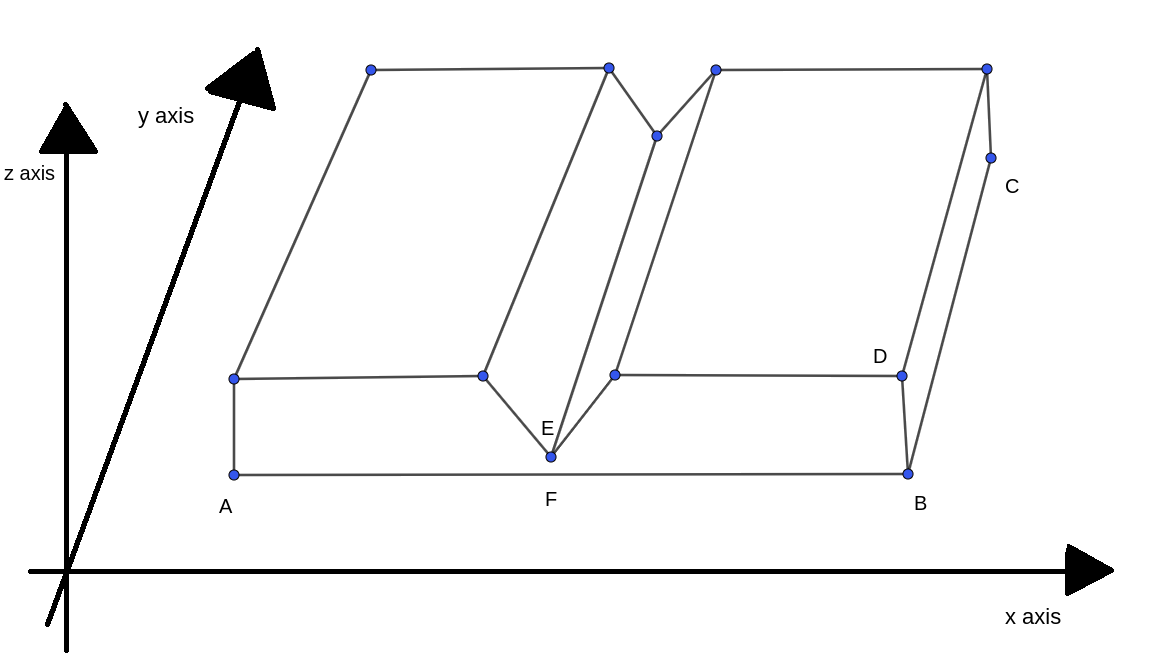
\includegraphics[width=4.5in]{spectralcluster/images/counterexample.png}
\caption{
  The probability density function where $\rho(x, y) =
    \min(\epsilon + x, \frac{1}{n})$ for arbitrary $X, Y, n$.
      Here, $\rho(x,y)$ is plotted in the z axis, and $E$ is at point
      $(0, -Y, \epsilon)$. This function $\rho$ has bad spectral sweep
      cuts when $\alpha = 1, \gamma = 2$.
 }
\label{fig:counterexample}
\end{figure}

We note that this
section combined with Theorem~\ref{thm:sweep-cut},
Lemma~\ref{lem:cheeger-converse} and Lemma~\ref{lem:buser-converse} shows that no Cheeger and Buser
inequality can hold when $\alpha = 1$ and $\gamma = 2$ for any
$\beta$: this section combined with Theorem~\ref{thm:sweep-cut} will
show that the Cheeger-Buser inequalities can only hold for $\beta > 10$,
while Lemma~\ref{lem:cheeger-converse} and Lemma~\ref{lem:buser-converse} shows that they can only hold for
$\beta \leq 1$. Therefore, the Cheeger-Buser inequalities cannot hold for
any $\beta$, for $\alpha = 1$ and $\gamma = 2$.

% See Section~\ref{sec:trade-offs} for more details.

\begin{theorem}\label{thm:counterexample} \textbf{$(\alpha=1,\gamma=2)$-Spectral Sweep Cut Counterexample:}

  For a $1$-Lipschitz positive valued function $\rho$, let $\Phi$ be the
  sparsity of the $(1,3)$-spectral sweep cut, and let $\Phi_{OPT}$ be
  the cut of optimal $(1, \beta)$ sparsity for any $\beta < 10$. There
  there exists a $1$-Lipschitz density function $\rho$ such that:

  \[\Phi > C \max(\Phi_{OPT}, \sqrt{\Phi_{OPT}})\]
  for any constant $C$.
\end{theorem}

\subsection{Our density function}
We first construct our $1$-Lipschitz Density function for which a
$(1,2)$ spectral cut has poor $(1,\beta)$ sparsity. Our density function
has parameters $X, Y, \epsilon, n$ which we will set later.

\begin{definition} Let $\rho: [-X, X] \times [-Y, Y] \rightarrow \mathbb{R}$ be a density function such that:

  \[ \rho(x, y) = \min(\epsilon + x, 1/n) \] 
\end{definition}
To turn this into a $1$-Lipschitz probability density function, we simply
extend it to a function $\rho':\mathbb{R}^2 \rightarrow \mathbb{R}$
where $\rho'$ agrees with $\rho$ on $[-X, X] \times [-Y, Y]$, and the
function goes $1$-Lipschitzly to $0$ outside this range.

We will set $X = \sqrt{n}/10, Y = 10\sqrt{n}$, and $n$ large, to obtain
a density function where the $(1, 2)$ spectral cut has arbitrarily bad
$(1,\beta)$ sparsity for all $\beta < 10$. 

\subsection{Proof Overview}

First, we prove theorems about the zero-set of this density's
$(\alpha=1,\gamma=2)$ eigenfunction. In particular, the zero-set of this
eigenfunction must cut from the line $x=-X$ to $x=X$. It cannot cut from
the line $y = -Y$ to the line $y = Y$.

We prove that any level-set of the eigenfunction can't cut from $y
= -Y$ to $y = Y$. We then show that any cut that doesn't cut from $y =
-Y$ to $y = Y$ has bad $(1,\beta)$ sparsity for $\beta < 10$. This
completes our proof. Moreover, any cut that doesn't cut from $y=-Y$ to
$y=Y$ is intuitively a poor cut of our density function, according to
standard machine learning intuition.

We note the natural cut of this distribution is the straight line cut $x =
0$, which the $(1,3)$-spectral sweep cut will find (this is an artifact
of our proof, though we do not explicitly prove it here).

First, we prove a few lemmas on the zero-set of the $(1,2)$
eigenfunction.
\subsection{The Zero-set of a principal $(1,2)$ eigenfunction is the
line $y = 0$} 

\begin{theorem} \label{thm:zero-set} The Zero-set of the eigenfunction for our given density
  function, is the line $y = 0$.
\end{theorem}
\begin{lemma} Let $f$ be any eigenfunction of our given density function,
  for which $f(x,y) \not= f(x, y')$ for some $x, y \not= y'$. Then
  
  \[ \int_0^Y f(x,y) dy  = 0. \]
\end{lemma}

\begin{lemma}\label{lem:symmetry} There exists a principal eigenfunction $f_2$ of our given
  density function, for which 

  \[f_2(x,y) = f_2 (-x, y) = -f_2(x,-y)\]

\end{lemma}

\begin{proof} This follows from a (non-trivial) symmetrization argument put forward in
  the graph case in Guattery and Miller~\cite{GuMi95}.
\end{proof}

\begin{lemma}\label{lem:nodal} (Nodal domains for Densities) Every principal eigenfunction $f_2$ of our given density
  function satisfies: the closure of the set $\{S = (x,y) | f_2(x,y)
  > 0\}$ is connected.
\end{lemma}
\begin{proof} This follows analogously to the proof of Fiedler's nodal
  domains for eigenfunctions of a graph~\cite{Fiedler73}.
\end{proof}

  \begin{lemma}  \label{lem:pos-neg} Let $f$ be a $(\alpha, \beta)$ eigenfunction of any density function
  supported on a compact set $S \subset \mathbb{R}^n$ for some $n$.
  For every point in the zero-set, if any open set containing that point
  contains a positive element, it must also contain a negative element.
\end{lemma}
\begin{proof}
  This follows directly from the definition of eigenfunction.
\end{proof}

  \begin{proof} (of Theorem~\ref{thm:zero-set}):
    First, we note that there is a principal eigenfunction whose zero
    set contains $y = 0$, by Lemma~\ref{lem:symmetry}. We claim there is a principal
    eigenfunction for which this is the entire zero-set. This follows
    from Lemma~\ref{lem:nodal} and Lemma~\ref{lem:pos-neg}.
  \end{proof}

%% TIM ENDED HERE.

\subsection{Any spectral sweep cut has high $(1,\beta)$ sparsity}
In this section, we prove that the spectral sweep cut must have high $(1,\beta)$-sparsity
for $0 < \beta < 10$, and for $\beta>10$ the spectral sweep-cut either
has high $(1,\beta)$ sparsity or else divides the probability density
into two pieces, one of which has less than $\leq 1/n$ fraction
of the probability mass. 

\begin{lemma}~\label{lem:not-vertical} Any spectral sweep cut (of the principal $(1,2)$
  eigenfunction whose eigenvector's zero-set is the line $y = 0$) can't cut through $y=Y$ and $y =
  -Y$.
\end{lemma}
\begin{proof} 
  This is clear.
\end{proof}
\begin{lemma}\label{lem:notsparse} Any cut that doesn't cut through both $y=Y$ and $y=-Y$ has
  poor $(1,\beta)$ sparsity for any $0 < \beta < 10$. For $\beta > 10$,
  a cut of good $(1,\beta)$ sparsity must have its smaller side contain $o_n(1)$ fraction of the
  mass. 
  
  To be precise, if $\Phi_{\beta}$ is the optimal $(1,\beta)$
  sparsity of the cut, and $\Phi$ is the $(1,\beta)$ sparsity induced by
  a cut that doesn't cut both $y=Y$ and $y=-Y$, then there is no
  constant $C$ independent of $n$ for which

  $\Phi^2 <  C \Phi_\beta $.
\end{lemma}
We note that Theorem~\ref{thm:counterexample} follows from
Lemma~\ref{lem:not-vertical} and~\ref{lem:notsparse}. Thus, it remains
to show Lemma~\ref{lem:notsparse}.

\begin{proof} (of Lemma~\ref{lem:notsparse}). We split this into two
  cases. Consider the side of the level set cut with smaller probability
  mass. The first case is when this side has at least half its
  probability mass outside the region $|x| < 1/n-\epsilon$. The second case is when
  the side has less than half its mass in this region.

  In the first case, we note that we can lower bound the cut by its
  projection onto the $x$ axis. A quick calculation shows that when $X =
  \frac{1}{10\sqrt{n}}$ and $Y = \frac{10}{\sqrt{n}}$, the $(1,
  \beta)$-sparsity of this cut is within a factor of $2$ of the $(1,
  \beta)$-sparsity of the cut $y = 0$ through the uniform distribution of height
  $\frac{1}{n}$ supported on $[-X, X] \times [-Y, Y]$. This $(1, \beta)$
  sparsity is 
  \[ A:= O(\frac{X}{n^\beta}) = O(\frac{\sqrt{n}}{n^\beta})
  \].

  When $\epsilon$ is chosen to be $\frac{1}{n^2\sqrt{n}}$, then the
  $(1,\beta)$ sparsity of the optimal cut is the cut $x=0$, which has
  $(1,\beta)$ sparsity of:
  \[B:= O(\frac{Y}{(n\sqrt{n})^\beta}) =
  O(\frac{\sqrt{n}}{(n^2\sqrt{n})^\beta}.\]

  We note that this choice of $\epsilon$ is the minimum such choice such
  that the principal eigenvector is not constant on the $Y$ axis.

  Now we note that $A^2/B$ goes to infinity as $n$ gets large, if and
  only if

  \[ n^{2\beta} \sqrt{n}^\beta n / n^{2\beta} \sqrt{n} \] goes to infinity,

  or 
  \[ \sqrt{n} (\sqrt{n}^\beta)\] goes to infinity. This is true for any
  $\beta > 0$. This proves Theorem~\ref{thm:counterexample} in case $1$,
  where at least half of the probability mass is outside the region $|x|
  < 1/n$.

  In case $2$, we consider the  case when the smaller side of the cut
  has more than half its probability mass inside the region $|x| < 1/n
  -\epsilon$, which we note is a very small portion of the probability
  mass of the overall probability density. In
  this case, it turns out that we need $\beta < 10$ to give isoperimetry
  guarantees, since for any $\beta > 10$, it turns out that even cuts
  containing small probability mass are considered to have good
  $(1,\beta)$ sparsity, since for large $\beta$, $(1,\beta)$ sparse cuts
  tremendously favor small cuts, even if the smaller side has negligible
  probability mass.

  Since at least half the mass is inside the
  region $|x| < 1/n$, we can assume without loss of generality that the
  entire probability mass of the smaller side of the cut is inside this region, by simply projecting
  the cut onto this region (reducing its $\beta$-perimeter while
  decreasing probability mass by at most a factor of $2$). We can again
  use a symmetry argument analogous to~\ref{lem:symmetry} to show that
  any level set of this principal eigenfunction is symmetric about the
  $x$ axis (we note Lemma~\ref{lem:notsparse} is slightly stronger than
  this as it does not assume symmetry, but for our purposes we can
  strictly deal with symmetric cuts, and the non-symmetric case follows
  through a similar argument). 

  Now given the cut is symmetric about the $x$ axis, if the cut cuts
  through $(x',y')$, then it also cuts through $(-x',y')$, and we can lower
  bound the probability mass contained by the cut $y = y'$ with $x'
  \cdot \rho(x',y')$. A simple calculation using this estimate finishes
  the proof for us.


\end{proof}




%%%%%%%%%%%%%%%% OLD TEXT %%%%%%%%%%%%%%%%%%%%%%
% To prove that the continuous version of classical spectral clustering
% fails to find a $(1, \beta)$-sparse cut, we first establish structure
% about one of the principal eigenvector. In particular, we will show that there
% is a principal eignevector whose $0$-set has a nice structure: it will cut from
% $y=0$ to $y=X$, while the $0$-set cannot touch both $x = 0$ and $x=X$.
% We will show that a cut with the $0$-set as threshold will lead to a
% poor $(1,\beta)$-sparsity.
% Note that a spectral sweep-cut using any threshold $t$ must be contained
% strictly on either side of the cut, and thus cannot touch the two lines
% $x=0$ and $x=X$ simultaneously. We will then prove:
% 
% \begin{lemma} For the density function shown in
%   figure~\ref{fig:counterexample}, any cut that does not touch $x=0$ and
%   $x=X$ simultaneously must have $(1,\beta)$ sparsity of at most
%   $\epsilon^\beta n$ for all $\epsilon < 1/n$.
% \end{lemma}
% \begin{lemma} For $X = \Theta(Y)$, The optimal cut of the density function shown in
%   figure~\ref{fig:counterexample} has $(1,\beta)$ sparsity of
%   $\Theta(\epsilon^\beta \sqrt{n})$.
% \end{lemma}
% \begin{lemma} For $X = 10\sqrt{n}$, $Y = \sqrt{n}$, and $\epsilon \geq 
%   \frac{1}{n^2 \sqrt{n}}$, the principal $(\alpha=1,
%   \gamma=2)$-eigenfunction of the density funciton defined in
%   Definition~\ref{FOO2} has eigenvalue greater than $Q$.\tim{Define $Q$}.
% \end{lemma}
% 
% 
% \subsection{The principal Eigenvector's $0$-set cuts from $x = 0$ to $x
% = X$}
% 
% \subsection{The principal Eigenvector's $0$-set does not touch both $y =
% 0$ and $y=Y$}
% 
% \subsection{Any cut contained entirely within one side of the $0$-set
% has high $(1,\beta)$-sparsity}
